% Chapter 5

\chapter{Literature Study on Map Design and Data
  Visualization} % Main chapter title

\label{Chapter5} % For referencing the chapter elsewhere, use \ref{Chapter1} 

\lhead{Chapter 5. \emph{Map Design}} % This is for the header on each page - perhaps a shortened title

%----------------------------------------------------------------------------------------
\subsection{Animated Maps}\label{anime}
Animated maps are proven to be more powerful in conveying the
spatial-temporal pattern than static maps~\cite{McEachern1998}.

In order to represent dynamic geographic processes, map animation is a
natural choice. It was introduced to the world of cartography in
1930s~\cite{Harrower2008}. The major application of animated maps
include: 1) demonstrating the dynamic process of geographic events
(weather maps in weather forecasting is such an example) 2) assisting
pattern recognition and knowledge development for scientific
researches. The study by Dorling and Openshaw is an example of 
application 2), where they discovered new leukaemia hotspots through
animated maps~\cite{Dorling1992}.

Animated maps are not superior to static maps, it is just they are
good at different aspects of information convey. The animated map is
advantageous in demonstrating the changes between frames rather than
the absolute value represented in each frame~\cite{Dorling1992}. It is
proved to be more powerful in convey the spatial-temporal pattern than
static map~\cite{McEachern1998}.

Harrower and Fabrikant mentioned that the chanllenge of using animated
maps is the overflow of information and the vulnerability to
distraction~\cite{Harrower2008}. One example mentioned by Harrower and
Fabrikant is the comparison of color on the map and that on the legend
becomes difficult for animated maps as a result of the changing of
images. They proposed the audio legend approach of strengthening
information convey with minimized
distraction~\cite{Harrower2008}. This might become one of the next
extensions of the current Dynamic Energy Map interface design.

They also suggested that the difference in time should have different
visual representations in data display~\cite{Harrower2008}. Peuquet
claimed that ``The development of temporal analytical capabilities in
GIS such as temporal queries requires basic topological structures in
both time and space''~\cite{Peuquet1994}. Thus the different spatial
representation seems to be a natural choice for adapting to different
temporal resolution and scale.

They classify time into two types: linear and cyclic. Upon this
consideration, the design of the current interface include both an
overall time navigation utility and time navigation utilities that
facilitate jumps with time steps corresponding to the natural period
of energy data, such as month, day and hour. This design choice
is anticipated to facilitate the representation of both linear changes
and periodical changes of energy usage in the community.

The level of user control of playback behavior of animated maps is
also debatable. Some claim providing the full freedom of adjusting
this feature can enhance pattern understanding~\cite{Nelson1998}. But
others argue that this control will reduce time animation to still
images and impair its ability in conveying temporal changes
~\cite{Lowe2004}. In the current dynamic map project, both the
interactive version and the non-interactive version is provided: the
non-interactive version (a map animation) is accessible through
\href{http://www.armechxyj.com/energy-mapping.html#redblueAnime3d}{here}. The
interactive version is provided as a stand-alone Python program.

\subsection{Spatial Temporal Data Analysis}\label{stDataAnalysis}
In order to better utilize the power of Dynamic Maps, one has to
understand the special features of spactial-temporal data and the
methods of how to use spactial-temporal data. This leads to the
literature study of the following section of spatial temporal data
analysis.

One temptation of analyzing spatial-temporal data is to aggregate them
into ``time periods'' and ``zonal entities'' and then use the static
analysis method to analyze the aggregated data~\cite{Dorling1992}. The
problem of this approach is 1) it increases the sensitivity
(i.e. minor changes in input causes dramatic changes in output) and 2)
it removes the ``dynamic'' feature of a dynamic.
map~\cite{Dorling1992}.

One layer of the goal of a space-time map is to make ``complex dynamic
process'' visible, in the hope of letting observers comprehend the
dynamics of data presented and to gain a general insight. Baring this
goal in mind, Dorling and Openshaw suggested a noise removal or data
smoothing in both the time and space dimension before the actual map
creation~\cite{Dorling1992}.

\section{Data Classification}\label{dataClassification}
In order to write the data classification routine for the
demonstration of dynamic energy map in the current study, the authors
conducted a brief survey of the commonly used GIS software for
commonly applied data classification method. The software surveyed in
the study include: ArcGIS~\cite{GIS_Jenks2014}, GRASS
GIS~\cite{GRASSGIS2008}, gvGIS~\cite{gvGIS2011}, and QGIS. The data
classification method adopted by the surveyed software in creating a
thematic map include: 1) equal interval, 2) quantile 3) Jenks 4)
Standard Deviation 5) pretty breaks 6) manual interval (use context
specific break point values). The common data classification method
shared by all surveyed instances are ``Equal Interval'', ``Quantile''
and ``User Defined''. Therefore we chose to implement the ``Equal
Interval'' and ``Quantile'' method in the current project.

\begin{table}[h!]
  \centering
  \begin{tabular}{r|c c c c c c}
    \hline
           & Equal Interval & Quantile & Jenks & Pretty Breaks & StDev & User Defined\\
    \hline
    ArcGIS &      o        &    o     &  o    & x &  o  &   o  \\
 GRASS GIS &      o        &    o     &  x    & x &  o  &   o  \\
     GVSIG &      o        &    o     &  o    & x &  x  &   o  \\
      QGIS &      o        &    o     &  o    & o &  o  &   o  \\
    \hline
  \end{tabular}
  \caption{Data Classification Method (o: yes, x: no)}
  \label{tab:classify}
\end{table}

\begin{comment}

``Data Visualization with Spacetime Maps'', Richard L. Brownrigg, 2005
(read further later on)

\grey{To be continued later:
\begin{enumerate}[label*=\arabic*.]
\item ``Geographic Visualization: Designing Manipulable Maps for
    Exploring Temporally Varying Georeferenced Statistics'', MacEachren et al.\
\item ``Strategies for the Visualization of Geographic Time-Series
    Data'', Mark Monmonier, 2011
\item ``Evaluation of Methods for Classifying Epidemiological Data
    on Choropleth Maps in Series'', Brewer and Pickle, 2002
\end{enumerate}}
\end{comment}



However, the level of user control of playback behavior is debatable
according to previous literature about animated maps. Some claim
providing the full freedom of adjusting this feature can enhance
pattern understanding~\cite{Nelson1998}. But others argue that this
control will reduce time animation to still images and impair its
ability in conveying temporal changes ~\cite{Lowe2004}.



\section{not sure if to include}

\subsection{Specification of the Major Operation}
The desired major operations for the target user include: 
\begin{itemize}
\item Map display and careful choice of default settings for
  choropleth map display
\item Navigation utilities that navigates through dynamic map and data
  plot
\item Provide various plot routines that supplies quantitative
  information
\end{itemize}

\subsubsection{Map display and data plot}
Although the major target user group for the current project is
researchers and planners, we can briefly discuss an interface for
public user for future extending the project to adatp to different
user groups' need. In the study of Resch et al.\ suggest that the
interface for general public should ``ensure that the amount of
information shown to the users at any given time, and its complexity,
are reduced''~\cite{Resch2014}. Thus we could imagine the desired map
display for the current project should be a 3D map. The bivariate
choropleth map legend should also be replaced with two color ramps or
even with only colors of extreme value. Quantitative information
display should be reduced to one bar chart or zoomable data plot of
the aggregated demand. The data classification method should also be
chosen so that the peak occurrence time is emphasized rather than the
absolute energy consumption value. One sample design for such a map is
shown in \fref{fig:forPublic} (The data plot is not added in this
example).

  \begin{figure}[h!]
    \centering
    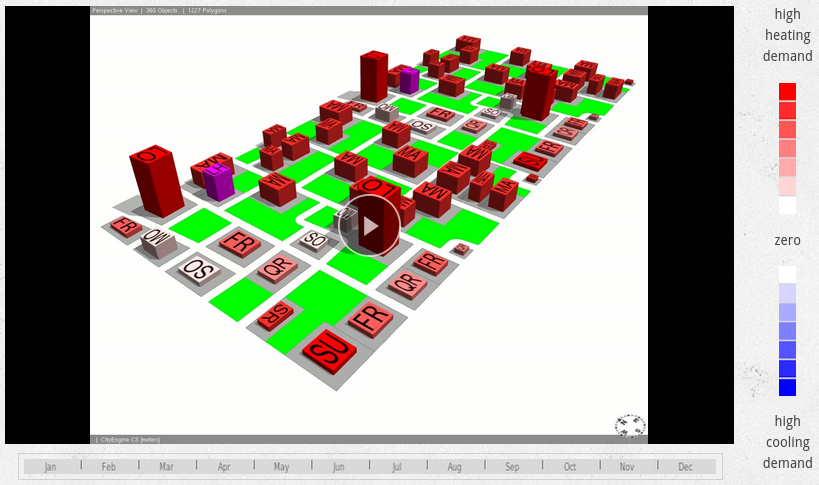
\includegraphics[width=0.7\linewidth]{forPublic.png}
    \caption[Animated Map for Public]{This version of animated map
      aims at revealing the dynamic changes of building heating and
      cooling energy demand and their non-conincident heating and
      cooling peak arrival for general public}
    \label{fig:forPublic}
  \end{figure}
  
For researchers or planners: The desired map display should be a 2D
and 3D map. They can toggle between the two display mode and can
perform different operations. The heating or cooling demand are
represented as a graduated symbol (univariate case) or color
(bivariate case). The map display should also be coupled with
corresponding data plot or data statistics that provides the
quantitative insight that supports design decisions.

\subsubsection{Navigation utilities that navigates through dynamic map
  and data plot}
The ability to navigate through a series of map images and present
dynamic data plot accordingly, is the basic function that differs
the current work from a static map. Some desired behavior of the
slider includes:

\begin{itemize}

\item Linear and cyclic time representation. According to section
  \ref{anime}, the time has both linear and cyclic aspect. The time
  navigation utility should provide both ``linear'' time navigation
  and ``cyclic'' time navigation. This requires a global time
  navigation that accounts for the linear aspect: it can go through
  the whole time period with the highest time resolution. It also
  requires a series of default time steps settings corresponding to
  the natural recurring pattern of the energy usage profile
\item Another desired feature is providing adjustable auto-play of the
  map animation. The reasoning behind this is the debatable level of
  user control in the study of Johnson and Nelson~\cite{Nelson1998},
  when they argue that allowing arbitrary time control might degrade
  the ability of animated map on conveying temporal pattern. This
  feature is to be implemented in future development of the project.
\end{itemize}

\subsection{Provide default settings for choropleth map display}
Creating several default settings for choropleth map display,
i.e. provide choices for data classification and color mapping. For
the current implementation, the variables in display is the heating
and cooling energy consumption profile. The customization choices only
restrict to the two classification method: even or quantile
method. The color ramp is predefined to be a bivariate color ramp from
white to red and blue. For later stages, a desired behavior would be
to provide the full control of color settings.


Dong et al.\ assessed the effectiveness of symbol design and frame
rate on the effectiveness of dynamic map display with two performance
measurements: deviation and response time. They identified the optimal
class numbers is 15 for graduated size symbol and is 10 for graduated
color symbol on a 1024x768 display. The optimal frame rate identified
in the study is 3 for color symbol maps and 6 for size symbol
maps. They also suggest to reduce class number and frame rate if the
display size is smaller than
1024x768~\cite{doi:10.1559/1523040639298}. 
